%\subsection{Estimating Bathymetry}

In this Section, we describe some experimental results with simulated and real data using few existing nonlinear optimization tools that we used in our preliminarily experiments (see Section \ref{inv_techniques}). Note that our forward model is nonlinear as described in Section \ref{forwardproblem} and it can not be written as a matrix equation system. Therefore, in this Bathymetry inversion, we can not use any inverting method where it needs forward operator as a explicit matrix operator (e.g., \verb|tikhonov| and  \verb|lsqnonneg|     
 Matlab\textsuperscript{\textregistered} functions need forward operator as a matrix). Moreover, the bounds of the true Bathymetry range in the interested near shore region is known to be $[0m, 11m]$. Therefore, we picked the inverse solvers that enables us to incorporate that prior knowledge too. 

\subsection{Simulated Data}
In this study, Gaussian noise corrupted simulated wave numbers (see Section \ref{Gaussian_noise} for more details) are generated by 
\begin{equation}
\mathbf{k}_s = A(\mathbf{h}_t) + \mathcal{N}(0, \nu^2),
\end{equation}
where $A(\cdot)$ represents the nonlinear forward operator defined in Section \ref{forwardproblem}, $\mathbf{h}_t \in \mathbb{R}_+^n$ is the true Bathymetry vector, and $\mathcal{N}(0, \nu^2)$ is a additive Gaussian noise vector with standard deviation $\nu$, generated in the Matlab\textsuperscript{\textregistered} by $\nu \cdot $\verb| randn(n,1)|. we manufactured wave numbers $\mathbf{k}_s$ for two different grid resolutions, i.e., 10m and 25m (see Fig. \ref{Simulated10m} and \ref{Simulated25m} respectively), to test and tune our inverse methods before working with actual measurements. 



\begin{figure}[H]
\center
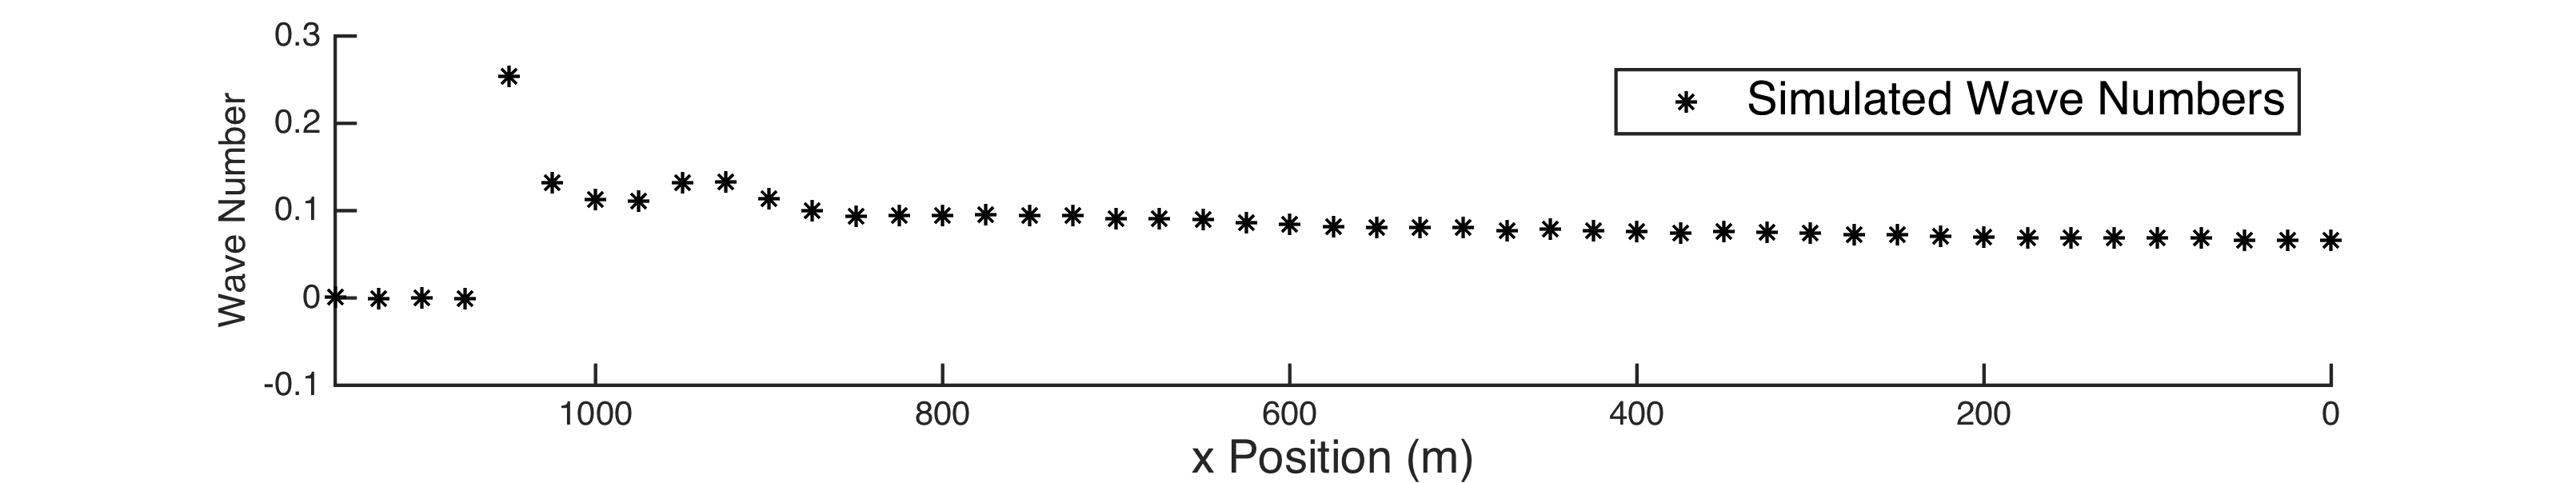
\includegraphics[scale=0.6]{img/simulated_data_k25m.png} 
\caption{1\% noisy ($\nu = 10^{-3}$) simulated wave numbers $(k)$ with 25m grid resolution. Noise (\%) = $\|A(\mathbf{h}_t) -  \mathbf{k}_s\| / \|  \mathbf{k}_s \| \cdot 100$.}
\label{Simulated25m}
\end{figure}

\begin{figure}[H]
\center
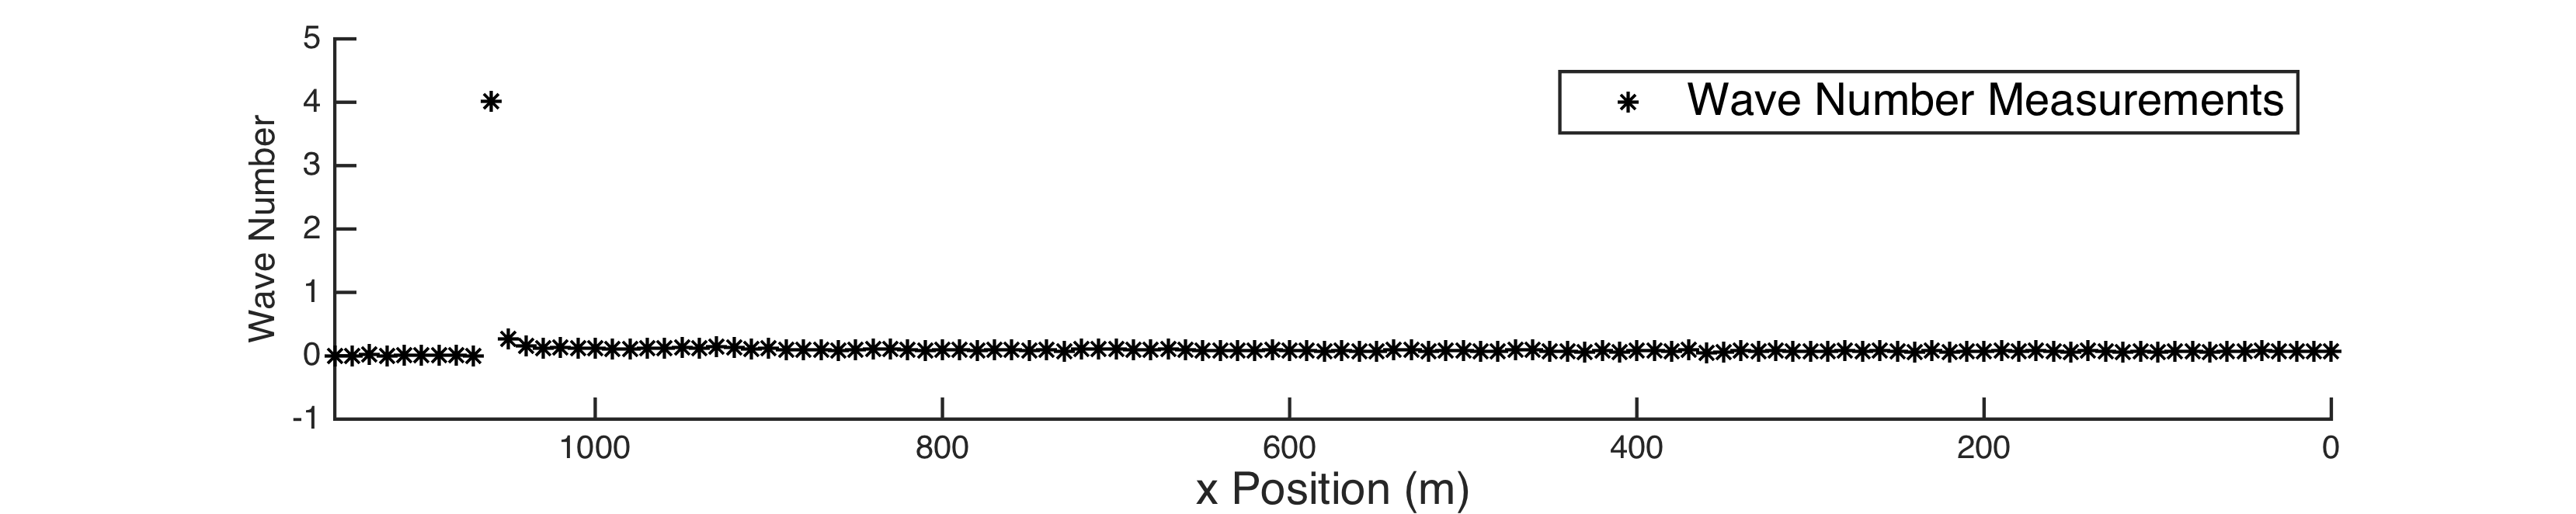
\includegraphics[scale=0.6]{img/simulated_data_k10m.png} 
\caption{2.5\% ($\nu = 10^{-2}$) noisy simulated wave numbers $(k)$ with 10m grid resolution. Noise (\%) = $\|A(\mathbf{h}_t) -  \mathbf{k}_s\| / \|  \mathbf{k}_s \| \cdot 100$. }
\label{Simulated10m}
\end{figure}


\subsection{Real Data}


Measured wave numbers (see Fig. \ref{RealData_oct09}) by US Army Corps of Engineers (USACE) at the field research facilities in Duck, NC on 09th October 2015  is used to approximate the true bathymetry using different inversion schemes. Note that the measured wave numbers near the shore (x Position $>$ 1050m) and the deep end (x Position $<$ 350m) are not available for our numerical experiments. 

\begin{figure}[H]
\center
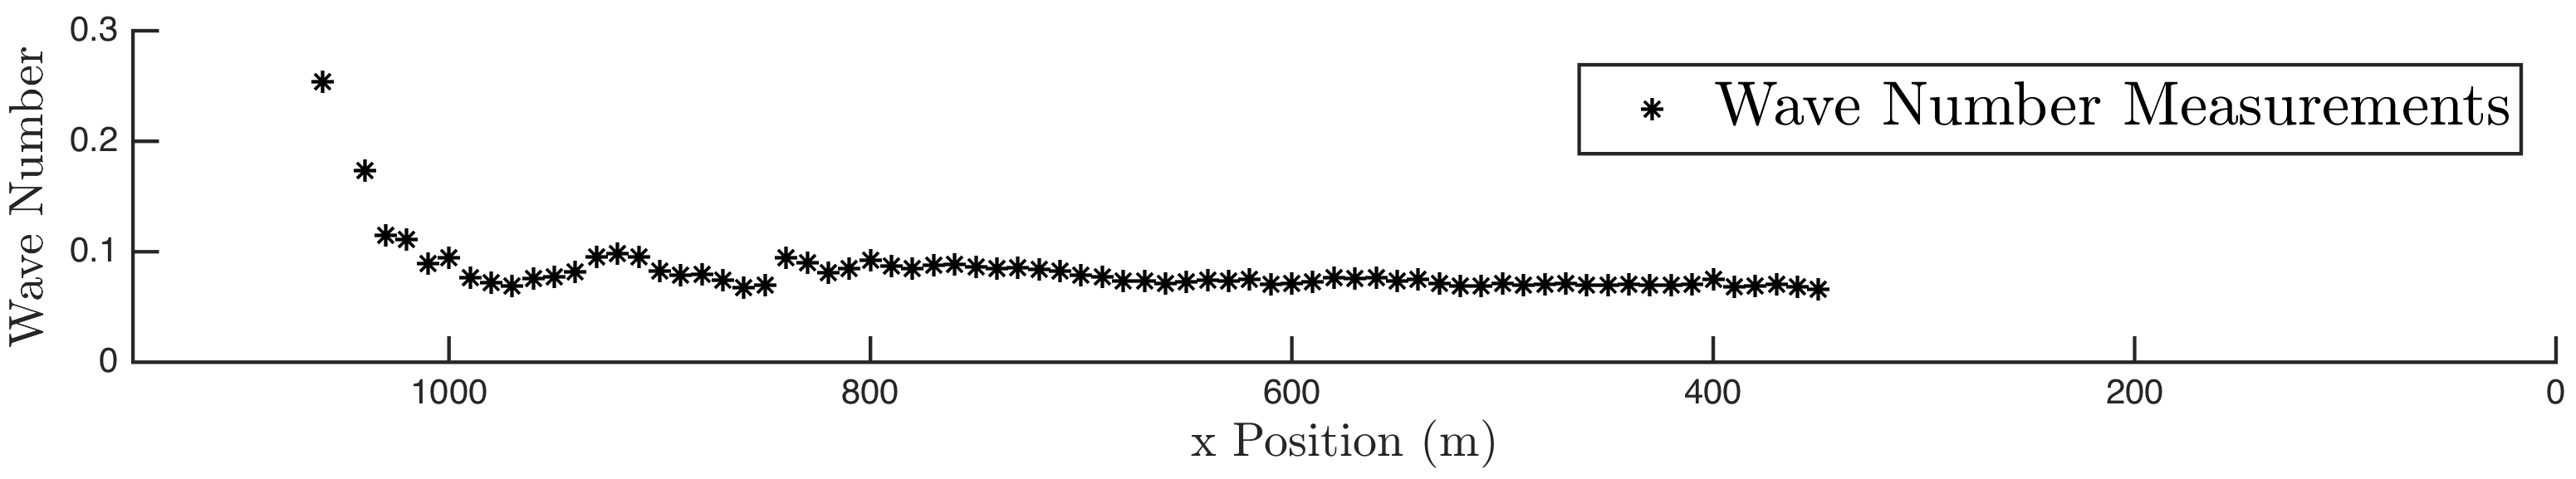
\includegraphics[scale=0.5]{img/real_data_k_Oct09.png} 
\caption{Real measurements of wave numbers $(k)$ on the 09th October 2015 at 21:59 by the US. Army Corps of Engineers (USACE) Engineer Research and Development Center (ERDC).}
\label{RealData_oct09}
\end{figure}




\subsection{Ordinary Least-Squares Fitting}


\begin{equation}\label{LS-BC}
\mathbf{\hat{h}}= \underset{\mathbf{0} \preceq \mathbf{h} \preceq \mathbf{11} }{\arg \min} \ \  \|  \mathbf{A}(\mathbf{h}) -  \mathbf{d} \|_2^2,
\end{equation}

\begin{figure}[H]
\center
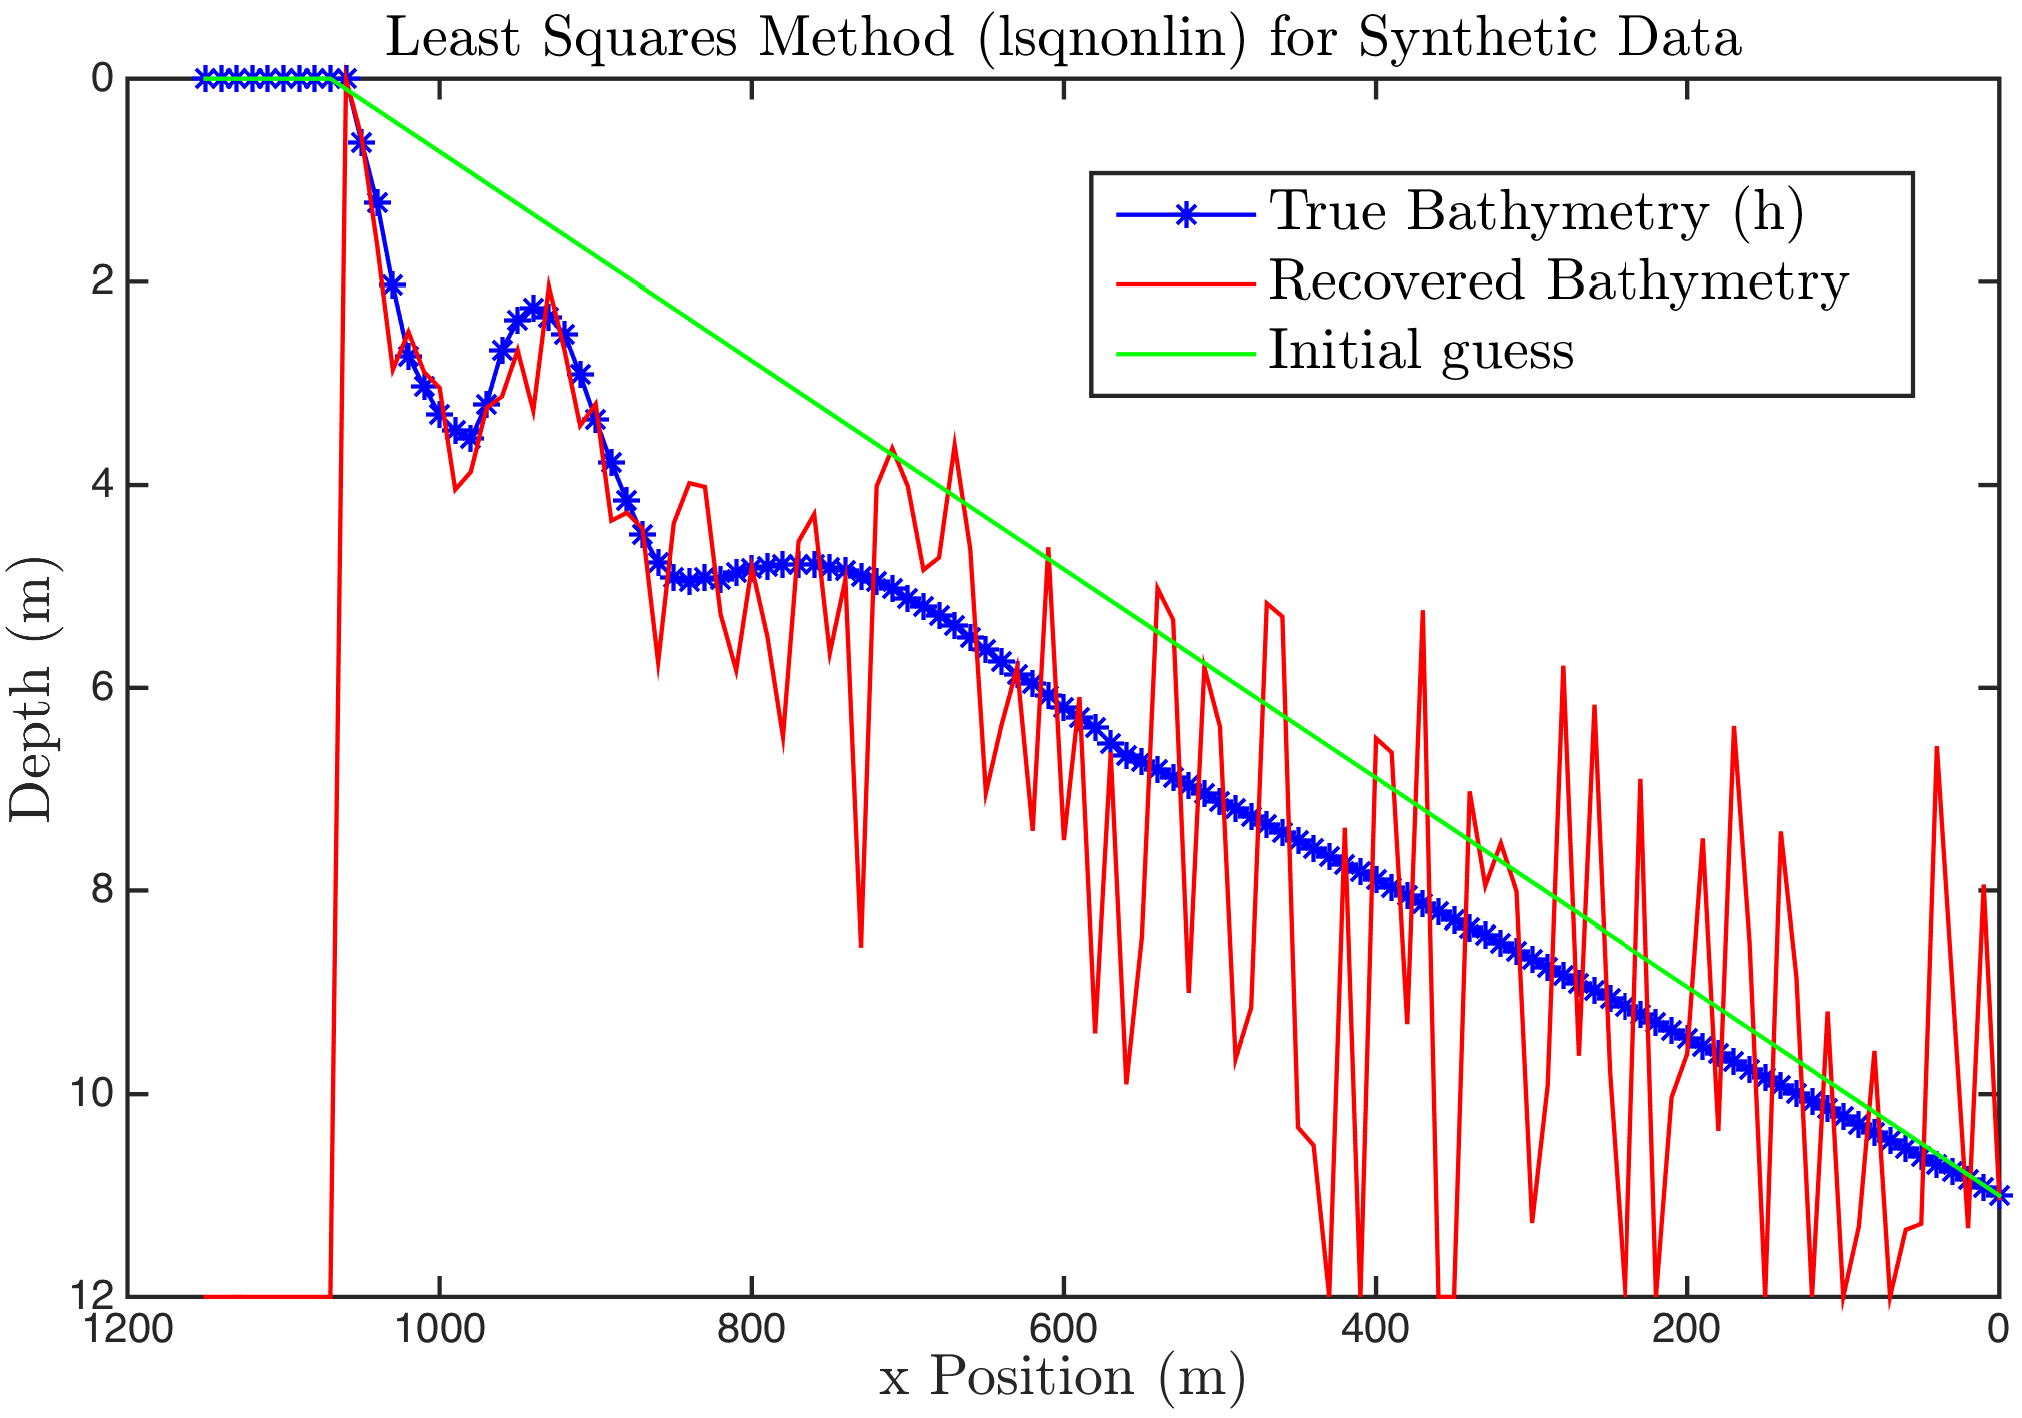
\includegraphics[scale=0.6]{img/lsqnonlin_simulated_10m.png} %plot20 
\caption{lsqnonlin method reconstruction of depth $\mathbf{h}$ using the simulated data.}
\label{fmincon_simulated}
\end{figure}

\begin{figure}[H]
\center
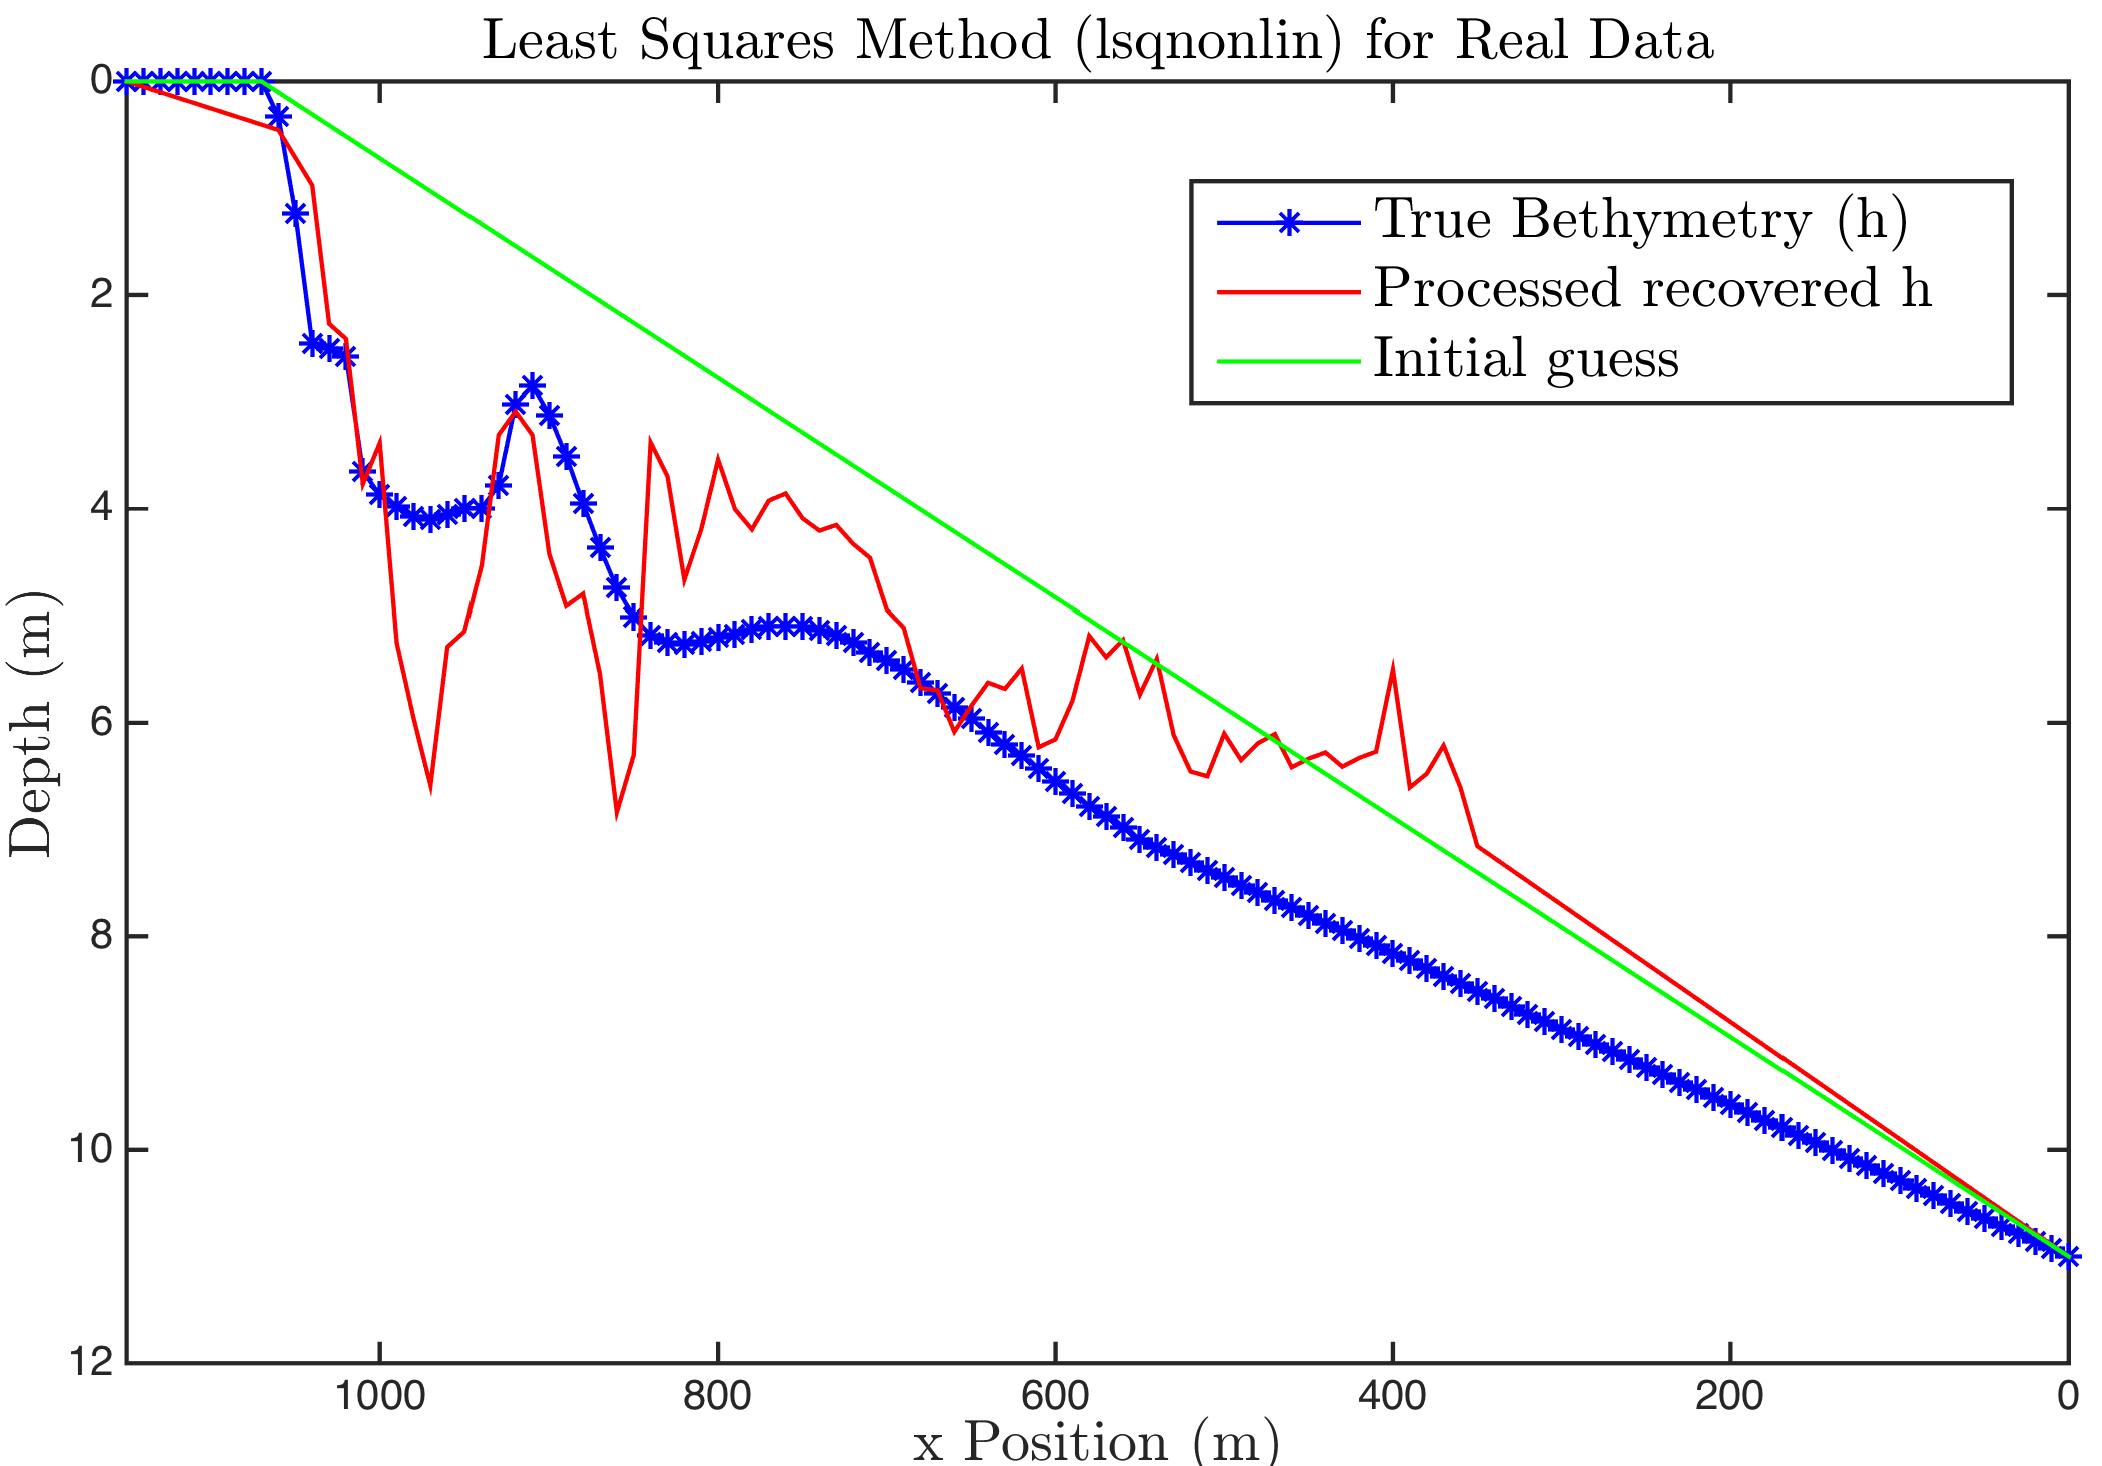
\includegraphics[scale=0.6]{img/lsqnonlin_real_data_oct09.png} %plot20 
\caption{lsqnonlin method reconstruction of depth $\mathbf{h}$ using the simulated data.}
\label{fmincon_simulated}
\end{figure}

\subsection{Tikhonov Regularization}

\begin{equation}\label{LS-regBC}
\mathbf{\hat{h}} = \underset{\mathbf{0} \preceq \mathbf{h} \preceq \mathbf{11}}{\arg \min} \ \ \|  \mathbf{A}(\mathbf{h}) -  \mathbf{d} \|_2^2  +  \alpha \| \mathbf{h}\|_2^2,
\end{equation}

[Using the Matlab's fmincon function ]


\begin{figure}[H]
\center
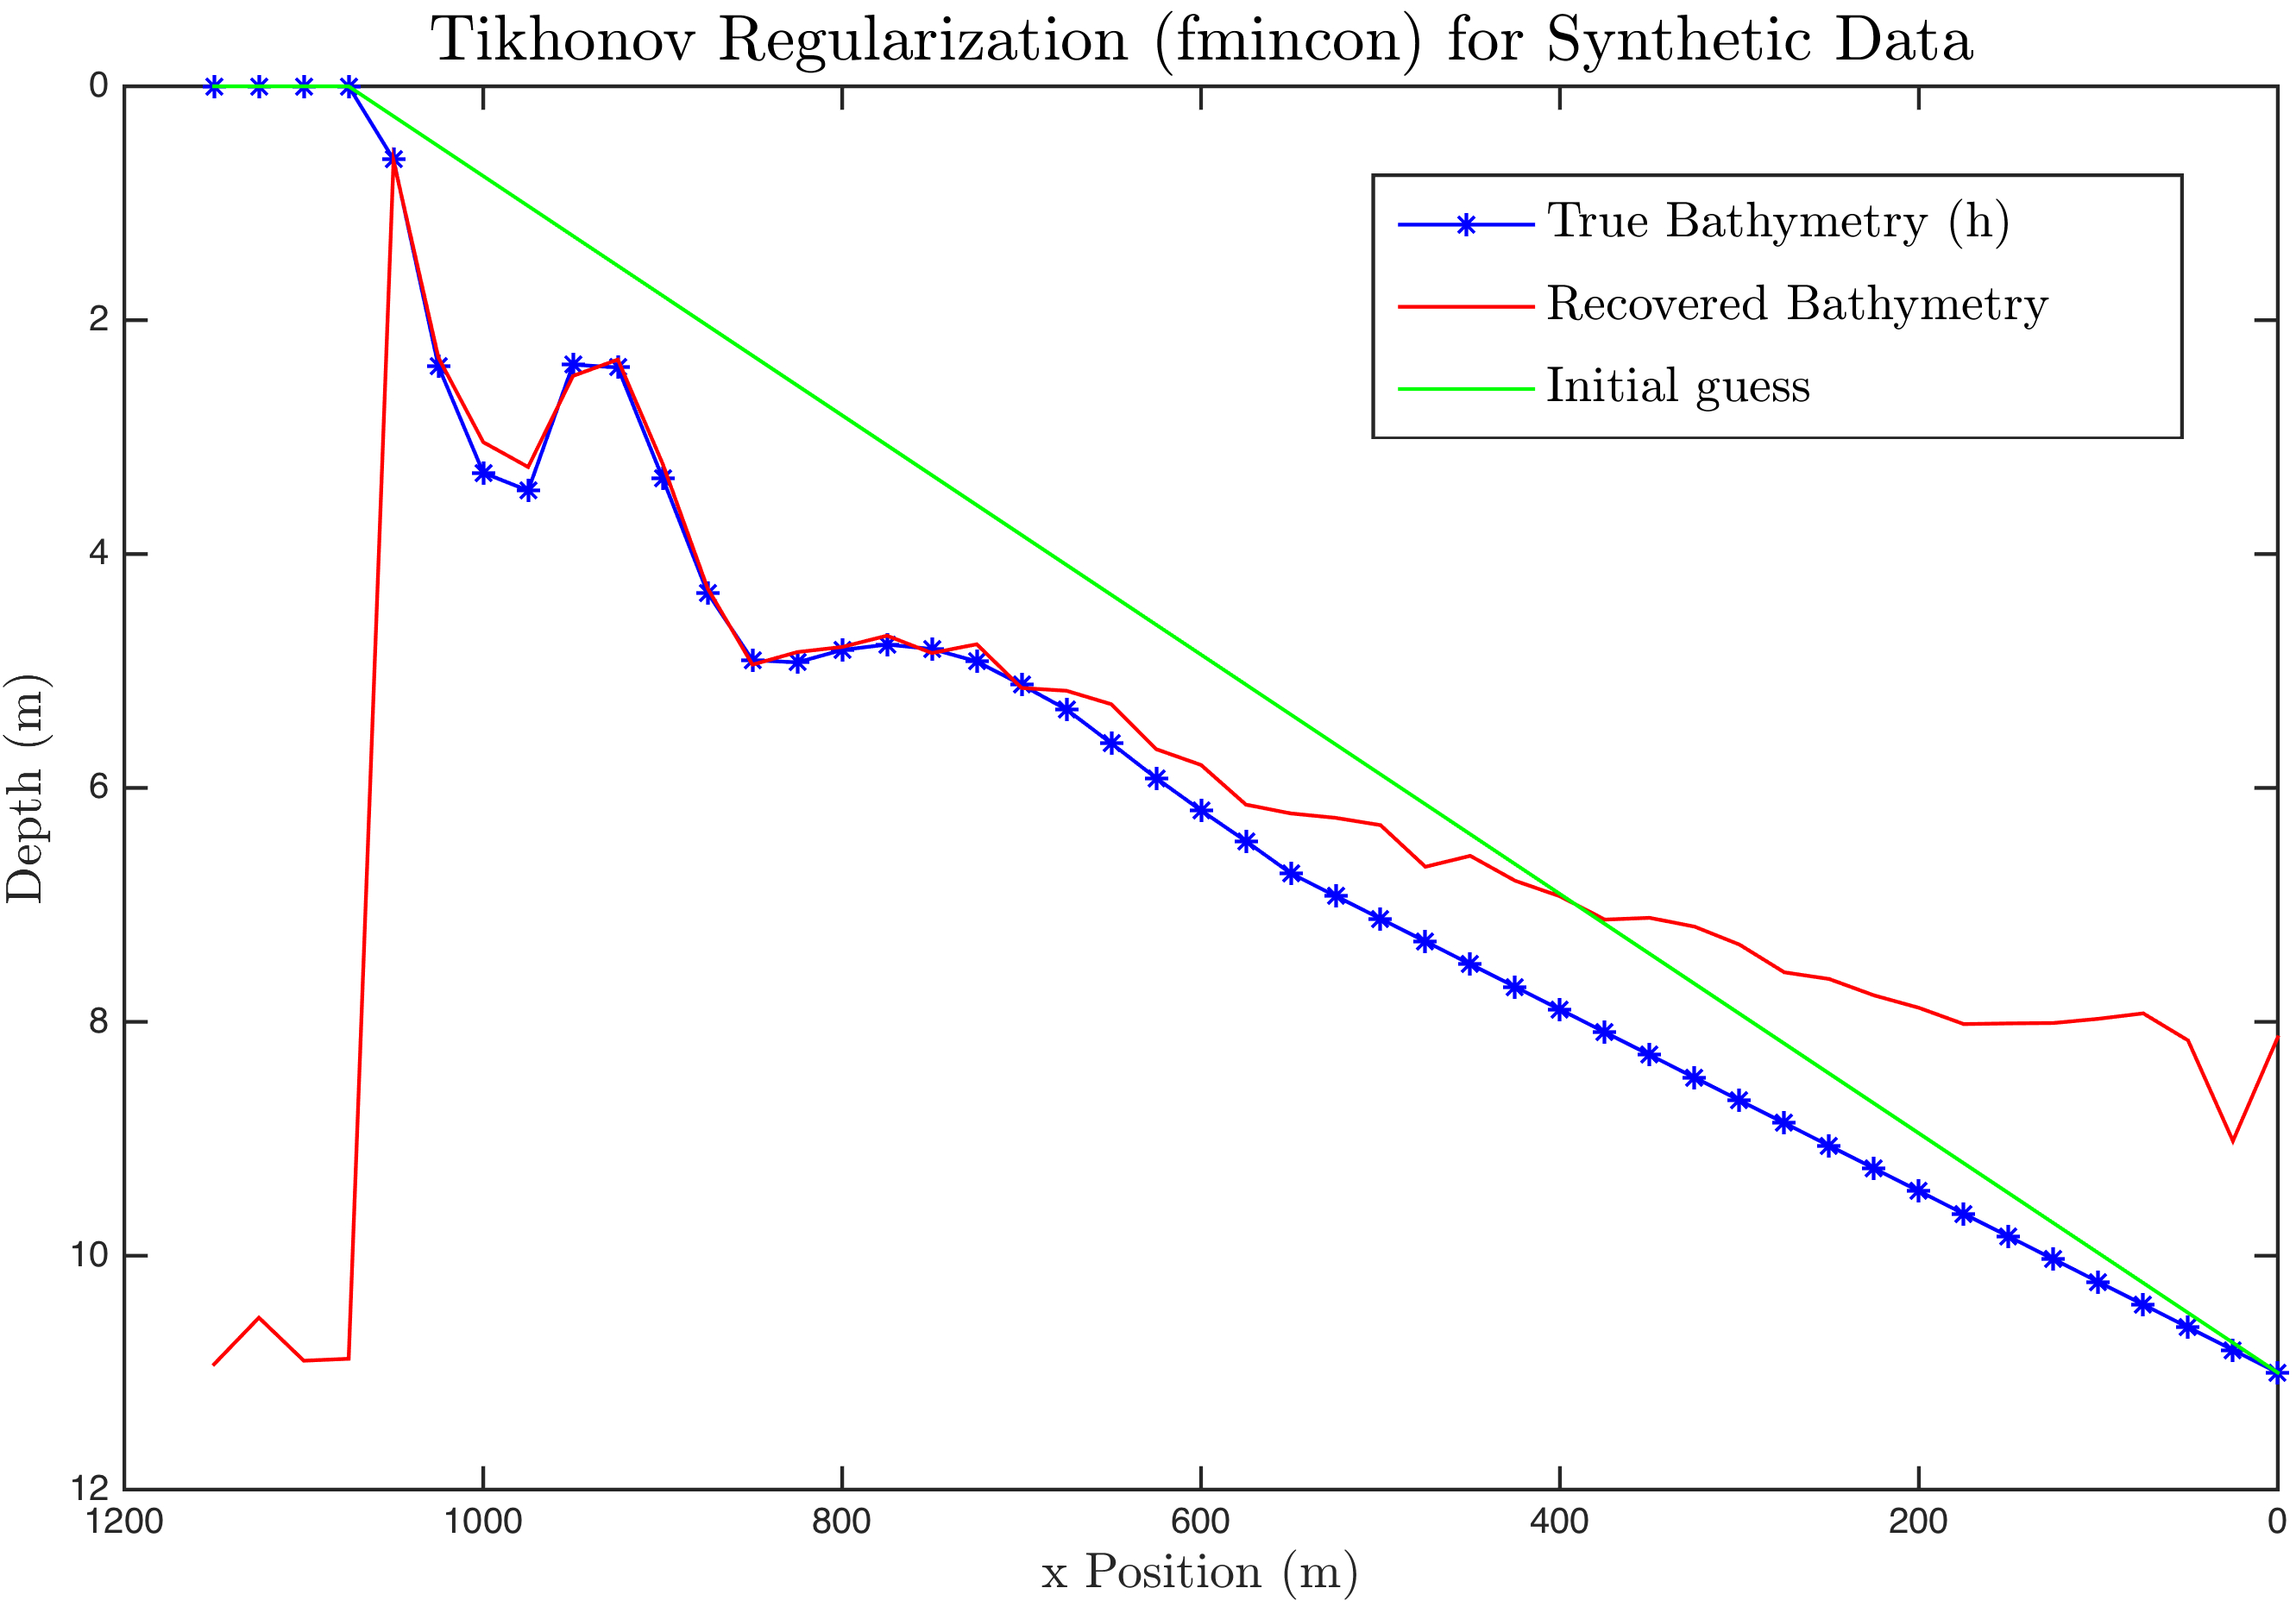
\includegraphics[scale=0.46]{img/fmincon_simulated_25m.png} %plot20 
\caption{fmincon method reconstruction of depth $\mathbf{h}$ using the simulated data.}
\label{fmincon_simulated}
\end{figure}

\begin{figure}[H]
\center
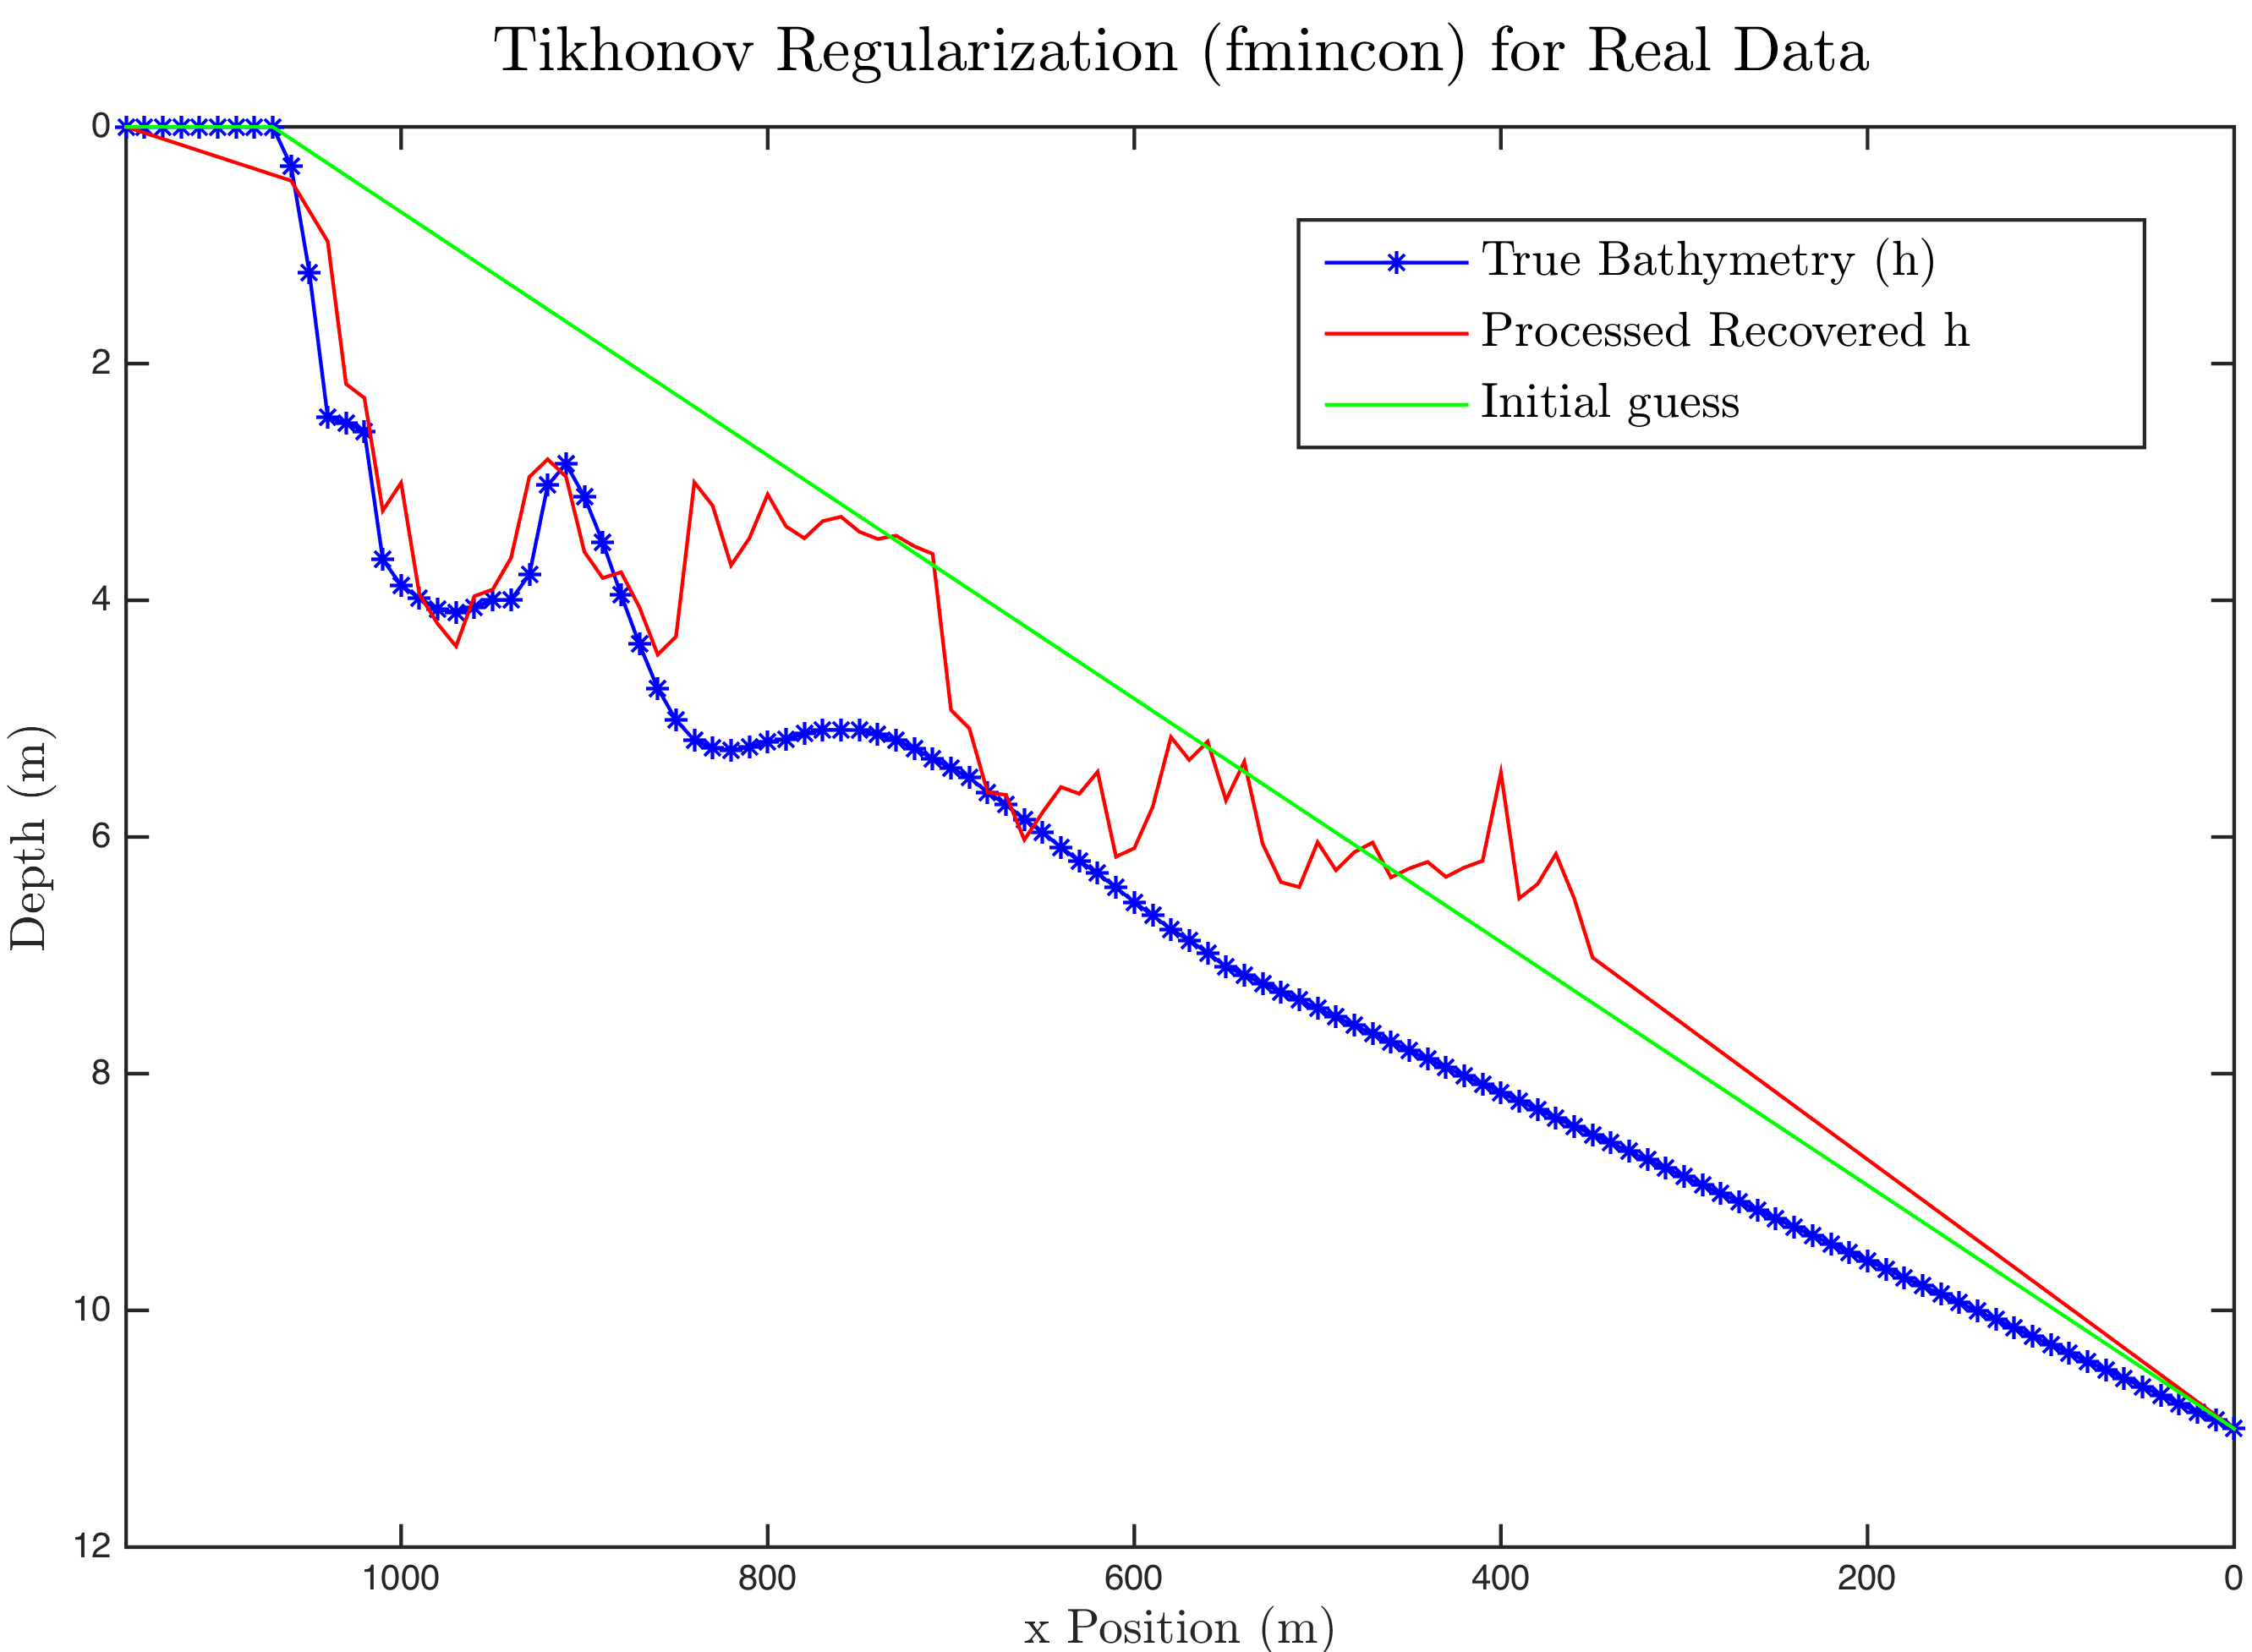
\includegraphics[scale=0.46]{img/fmincon_real_data_oct09.png} %plot20 
\caption{fmincon method reconstruction of depth $\mathbf{h}$ using the simulated data.}
\label{fmincon_simulated}
\end{figure}





